                                                                                                                                                                                                        % !TEX TS-program = pdflatex
% !TEX encoding = UTF-8 Unicode

% This is a simple template for a LaTeX document using the "article" class.
% See "book", "report", "letter" for other types of document.

\documentclass[11pt]{article} % use larger type; default would be 10pt

\usepackage[utf8]{inputenc} % set input encoding (not needed with XeLaTeX)
\usepackage{alltt}
\usepackage{listings}
\usepackage{graphicx}
\usepackage{amsmath}
\usepackage{float}
\newcommand*\diff{\mathop{}\!\mathrm{d}}

%%% Examples of Article customizations
% These packages are optional, depending whether you want the features they provide.
% See the LaTeX Companion or other references for full information.

%%% PAGE DIMENSIONS
\usepackage{geometry} % to change the page dimensions
\geometry{a4paper} % or letterpaper (US) or a5paper or....
% \geometry{margin=2in} % for example, change the margins to 2 inches all round
% \geometry{landscape} % set up the page for landscape
%   read geometry.pdf for detailed page layout information

\usepackage{graphicx} % support the \includegraphics command and options

% \usepackage[parfill]{parskip} % Activate to begin paragraphs with an empty line rather than an indent

%%% PACKAGES
\usepackage{booktabs} % for much better looking tables
\usepackage{array} % for better arrays (eg matrices) in maths
\usepackage{paralist} % very flexible & customisable lists (eg. enumerate/itemize, etc.)
\usepackage{verbatim} % adds environment for commenting out blocks of text & for better verbatim
\usepackage{subfig} % make it possible to include more than one captioned figure/table in a single float
\usepackage{amsmath}
% These packages are all incorporated in the memoir class to one degree or another...

%%% HEADERS & FOOTERS
\usepackage{fancyhdr} % This should be set AFTER setting up the page geometry
\pagestyle{fancy} % options: empty , plain , fancy
\renewcommand{\headrulewidth}{0pt} % customise the layout...
\lhead{}\chead{}\rhead{}
\lfoot{}\cfoot{\thepage}\rfoot{}

%%% SECTION TITLE APPEARANCE
\usepackage{sectsty}
\allsectionsfont{\sffamily\mdseries\upshape} % (See the fntguide.pdf for font help)
% (This matches ConTeXt defaults)

%%% ToC (table of contents) APPEARANCE
\usepackage[nottoc,notlof,notlot]{tocbibind} % Put the bibliography in the ToC
\usepackage[titles,subfigure]{tocloft} % Alter the style of the Table of Contents
\renewcommand{\cftsecfont}{\rmfamily\mdseries\upshape}
\renewcommand{\cftsecpagefont}{\rmfamily\mdseries\upshape} % No bold!



\title{Numerical Analysis Homework 3}
\author{Margaret Dorsey}
%\date{} % Activate to display a given date or no date (if empty),
         % otherwise the current date is printed 

\begin{document}
\maketitle

\section*{Problem 1}
\subsection*{Computation}

\subsection*{Verifying Correctness}

\section*{Problem 2}
\subsection*{5 Point Stencils}
\subsubsection*{First Derivative}
\begin{tabular}{c | c | c }
n & Average Absolute Error & Average Relative Error \\
\hline
10 & 0.367324 & 1.105306 \\
20 & 0.223943& 0.445905\\
30 &0.152942&  0.289964\\
100 & 0.048564 & 0.136987 \\
200 &0.038970 &0.084145\\
\end{tabular}\\
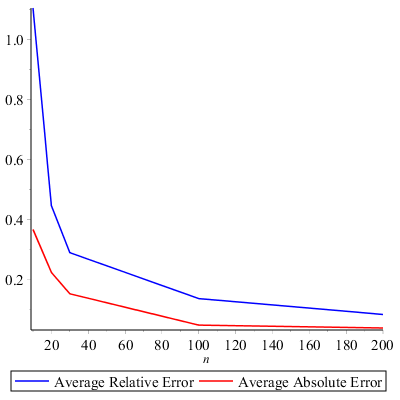
\includegraphics[scale=.5]{plots/problem2firstderivplot.png}
\subsubsection*{Second Derivative}
\begin{tabular}{c | c | c }
n & Average Absolute Error & Average Relative Error \\
\hline
10 & 0.745691 & 82151.805057 \\
20 & 2.315927& 22255.208023\\
30 & 0.312447& 16943.067463\\
100 & 1.473741 & 10594.331845 \\
200 & 6.611830 & 40690.086618 \\
\end{tabular}\\
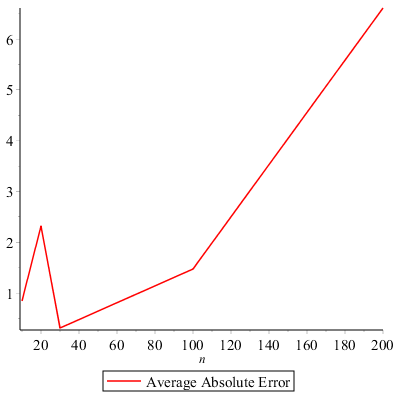
\includegraphics[scale=.5]{plots/problem2secondderivplot1.png}
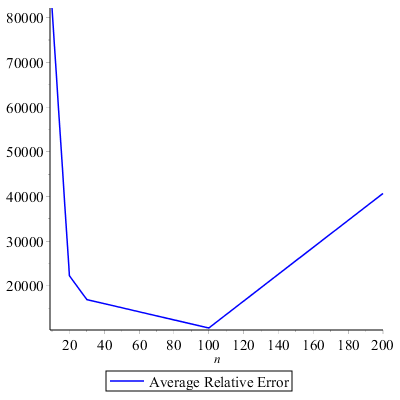
\includegraphics[scale=.5]{plots/problem2secondderivplot2.png}
\subsection*{Simpson's Rule}
Actual value of $\int_{0}^{\pi} \sin x \cdot e^{\cos x} dx$ : 2.350402.

\begin{tabular}{c | c | c }
n & Simpson's Result & Absolute Error \\
\hline
4 & 1.606199 & .744203 \\
10 & 2.215001 & .135401 \\
20 & 2.315927&  .034475\\
30 & 2.334574&  .015828\\
100 & 2.349178 & .001224 \\
200 & 2.350407 & .000005 \\
\end{tabular}

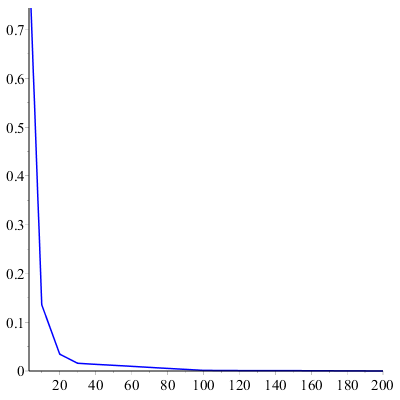
\includegraphics[scale=.5]{plots/problem2simpsonplot.png}
\subsection*{Analysis}
Simpson's method remained fairly stable despite the noise, with the error showing a clear exponential decay as $n$ increased,
and achieving $10^{-5}$ accuracy at $n=200$.

The first derivative using stencils did a little worse, with the error not only not decreasing as quickly with increasing $n$, but also seeming to level out in its decay as $n$ becomes large.

The second derivative suffered from huge relative error as the true value of the second derivative became small, and regardless of $n$, it seems as though the error in the second derivative approximation stayed consistent with (and amplified) the behavior of the noise.

Raw data for this problem can be found in the outputs directory.

\section*{Problem 3}
\begin{tabular}{c c}
Simpson's Method Integration & 0.316200 \\
Trapezoid Method Integration & 0.318500 \\
Total Emitted Energy from Magnitude Spline & $64.469777\cdot L_\odot$\\
Total Emitted Energy from Luminosity Spline & $64.476557\cdot L_\odot$\\
\end{tabular}\\

\subsection*{Analysis}
Given the number of points, the results of Simpson's Method and the Trapezoid Method are fairly comparable. Converting to luminosity before splining rather than after does not seem to have had a tremendous impact on the approximated result.

\section*{Problem 4}

\subsection*{Median Photon Energy}
\subsection*{Mean Photon Energy}
\subsection*{Standard Deviation in Wavelength}


\section*{Problem 5}
\begin{enumerate}[a.)]
\item $\int_{-1}^{1} \cos^2xdx$\\
Actual value: 1.4546 \\
Romberg 3,3 Value: 1.452126

\item $\int_{-\frac{3}{4}}^{\frac{3}{4}} x \ln(x+1) dx$\\
Actual value: .324332 \\
Romberg 3,3 Value: 0.322879

\item $\int_{1}^{4} \sin^2x - 2x\sin x +1 dx$\\
Actual value: 1.3668 \\
Romberg 3,3 Value: 1.315255

\item $\int_{e}^{2e} \frac{1}{x\ln x}dx$\\
Actual value: .52659\\
Romberg 3,3 Value: .525648
\end{enumerate}

\section*{Problem 6}






\end{document}
